% !TeX spellcheck = en_GB

In this chapter we want to show the different cost rasters, that were created from the same set of layers at different resolutions.
The Least Cost Path is estimated from this set of rasters.
In the last step the Least Cost Path is computed from the medium resolution rasters and compared with the Least Cost Paths computed from a high resolution raster.

\subsection{Cost Raster}\label{subsec:cost-raster}

The cost raster contains all the costs for the geographical region of the study area.
%%The surrounding of the study area, uses a no-data value and will not be use for the calculation of the Least Cost Path.
The different intermediate cost rasters in the study area are aggregated by the maximum function.
If the resolution is higher than the object size, then the effect of setting all~touched to True or False is limited.
If all~touched is set to True and any part of the pixel that is covered by the object, the whole pixel is attributed to the object.
This makes the object appear larger.
This can be seen in figure~\ref{fig:costs_5m}, which shows a detailed view of the costs for the village of Beverstedt.
 %% Due to the maximum aggregation of the costs, the average cost of the raster of all~touched true will be over estimated.
To set all~touched to False is a better description of the real size of the object for high resolution.

\begin{figure}
	\centering

	\subfloat[\centering All touched: True.]{{\includegraphics[width=.45\linewidth]{./images/CostRaster_5m_alT_v2_small.png} }}%
	\qquad
	\subfloat[\centering All touched: False.]{{\includegraphics[width=.45\linewidth]{./images/CostRaster_5m_alF_v2_small.png} }}%
	\caption{Part of the cost raster. Contrasting the for different settings of all~touched at a resolution of 5~m.}
	\label{fig:costs_5m}
\end{figure}

In contrast, if the resolution is smaller, all~touched set to False leads to a loss of information for smaller objects.
Since the default cost is much smaller than the average cost, this method underestimates the cost.
The figure~\ref{fig:costs_100m} shows, that for the resolution of 100 m, larger objects are still included in the map, but smaller objects, such as roads, are only partially included.
\begin{figure}
	\centering

	\subfloat[\centering All touched: True.]{{\includegraphics[width=.45\linewidth]{./images/CostRaster_100m_alT_v2_small.png} }}%
	\qquad
	\subfloat[\centering All touched: False.]{{\includegraphics[width=.45\linewidth]{./images/CostRaster_100m_alF_v2_small.png} }}%
	\caption{Part of the cost raster. Contrasting the different settings for all~touched at a resolution of 100~m.}
	\label{fig:costs_100m}
\end{figure}


\subsection{Least Cost Paths}\label{subsec:least-cost-paths}
For each resolution the Least Cost Paths were estimated with the all~touched set to False and True.

For the study, a starting point was chosen at a transformer about 6~km north of the container terminal Bremerhaven and an end point at a transformer in the southeast of the Osterholz county. 

The distance between the paths is calculated by the mean minimum distance.
For each vertex $P_i$ in the path $L_1$ the minimum distance between the vertex $P_i$ and the path $L_2$
is calculated and then the minimum distances are averaged (see equation~\ref{eq:1}).
\begin{equation}
	\label{eq:1}
	d_{mean} = \frac{1}{|L_1|} \sum_{i=1}^{n} d_{min}(P_i, L_2) \Bigr\vert P_i \in L_1
\end{equation}
This equation is used to measure the degree of similarity between the paths.
The distances are measured at the same resolution (different setting for all~touched), and same setting of all~touched (different resolution).

Table~\ref{tab:2} shows, that the distance between two paths decreases
with increasing resolution.
In addition, this tendency is depicted in figure~\ref{fig:paths_resolution} for the calculated cost paths of 5~m and 100~m resolutions.


At the same time, the differences in the aggregated costs remain almost constant.
Thus the difference between the aggregated costs per resolution decreases.
Setting all~touched to False underestimates and to True overestimates the costs.

\begin{figure}
	\centering

	\subfloat[\centering resolution of 5 m.]{{\includegraphics[width=.45\linewidth]{./images/LeastCostPaths_5m_v2_small.png} }}%
	\qquad
	\subfloat[\centering resolution of 100 m.]{{\includegraphics[width=.45\linewidth]{./images/LeastCostPaths_100m_v2_small.png} }}%
	\caption{Figures of the Least Cost Paths contrasting the paths for different resolutions. Paths with all~touched set to False are indicated by dashed lines and True are indicated by continuous lines. Higher resolutions are indicated by the color green, lower resolutions by the color red. Using OpenStreetMaps as base map.}
	\label{fig:paths_resolution}
\end{figure}

\begin{figure}
	\centering

	\subfloat[\centering all touched False.]{{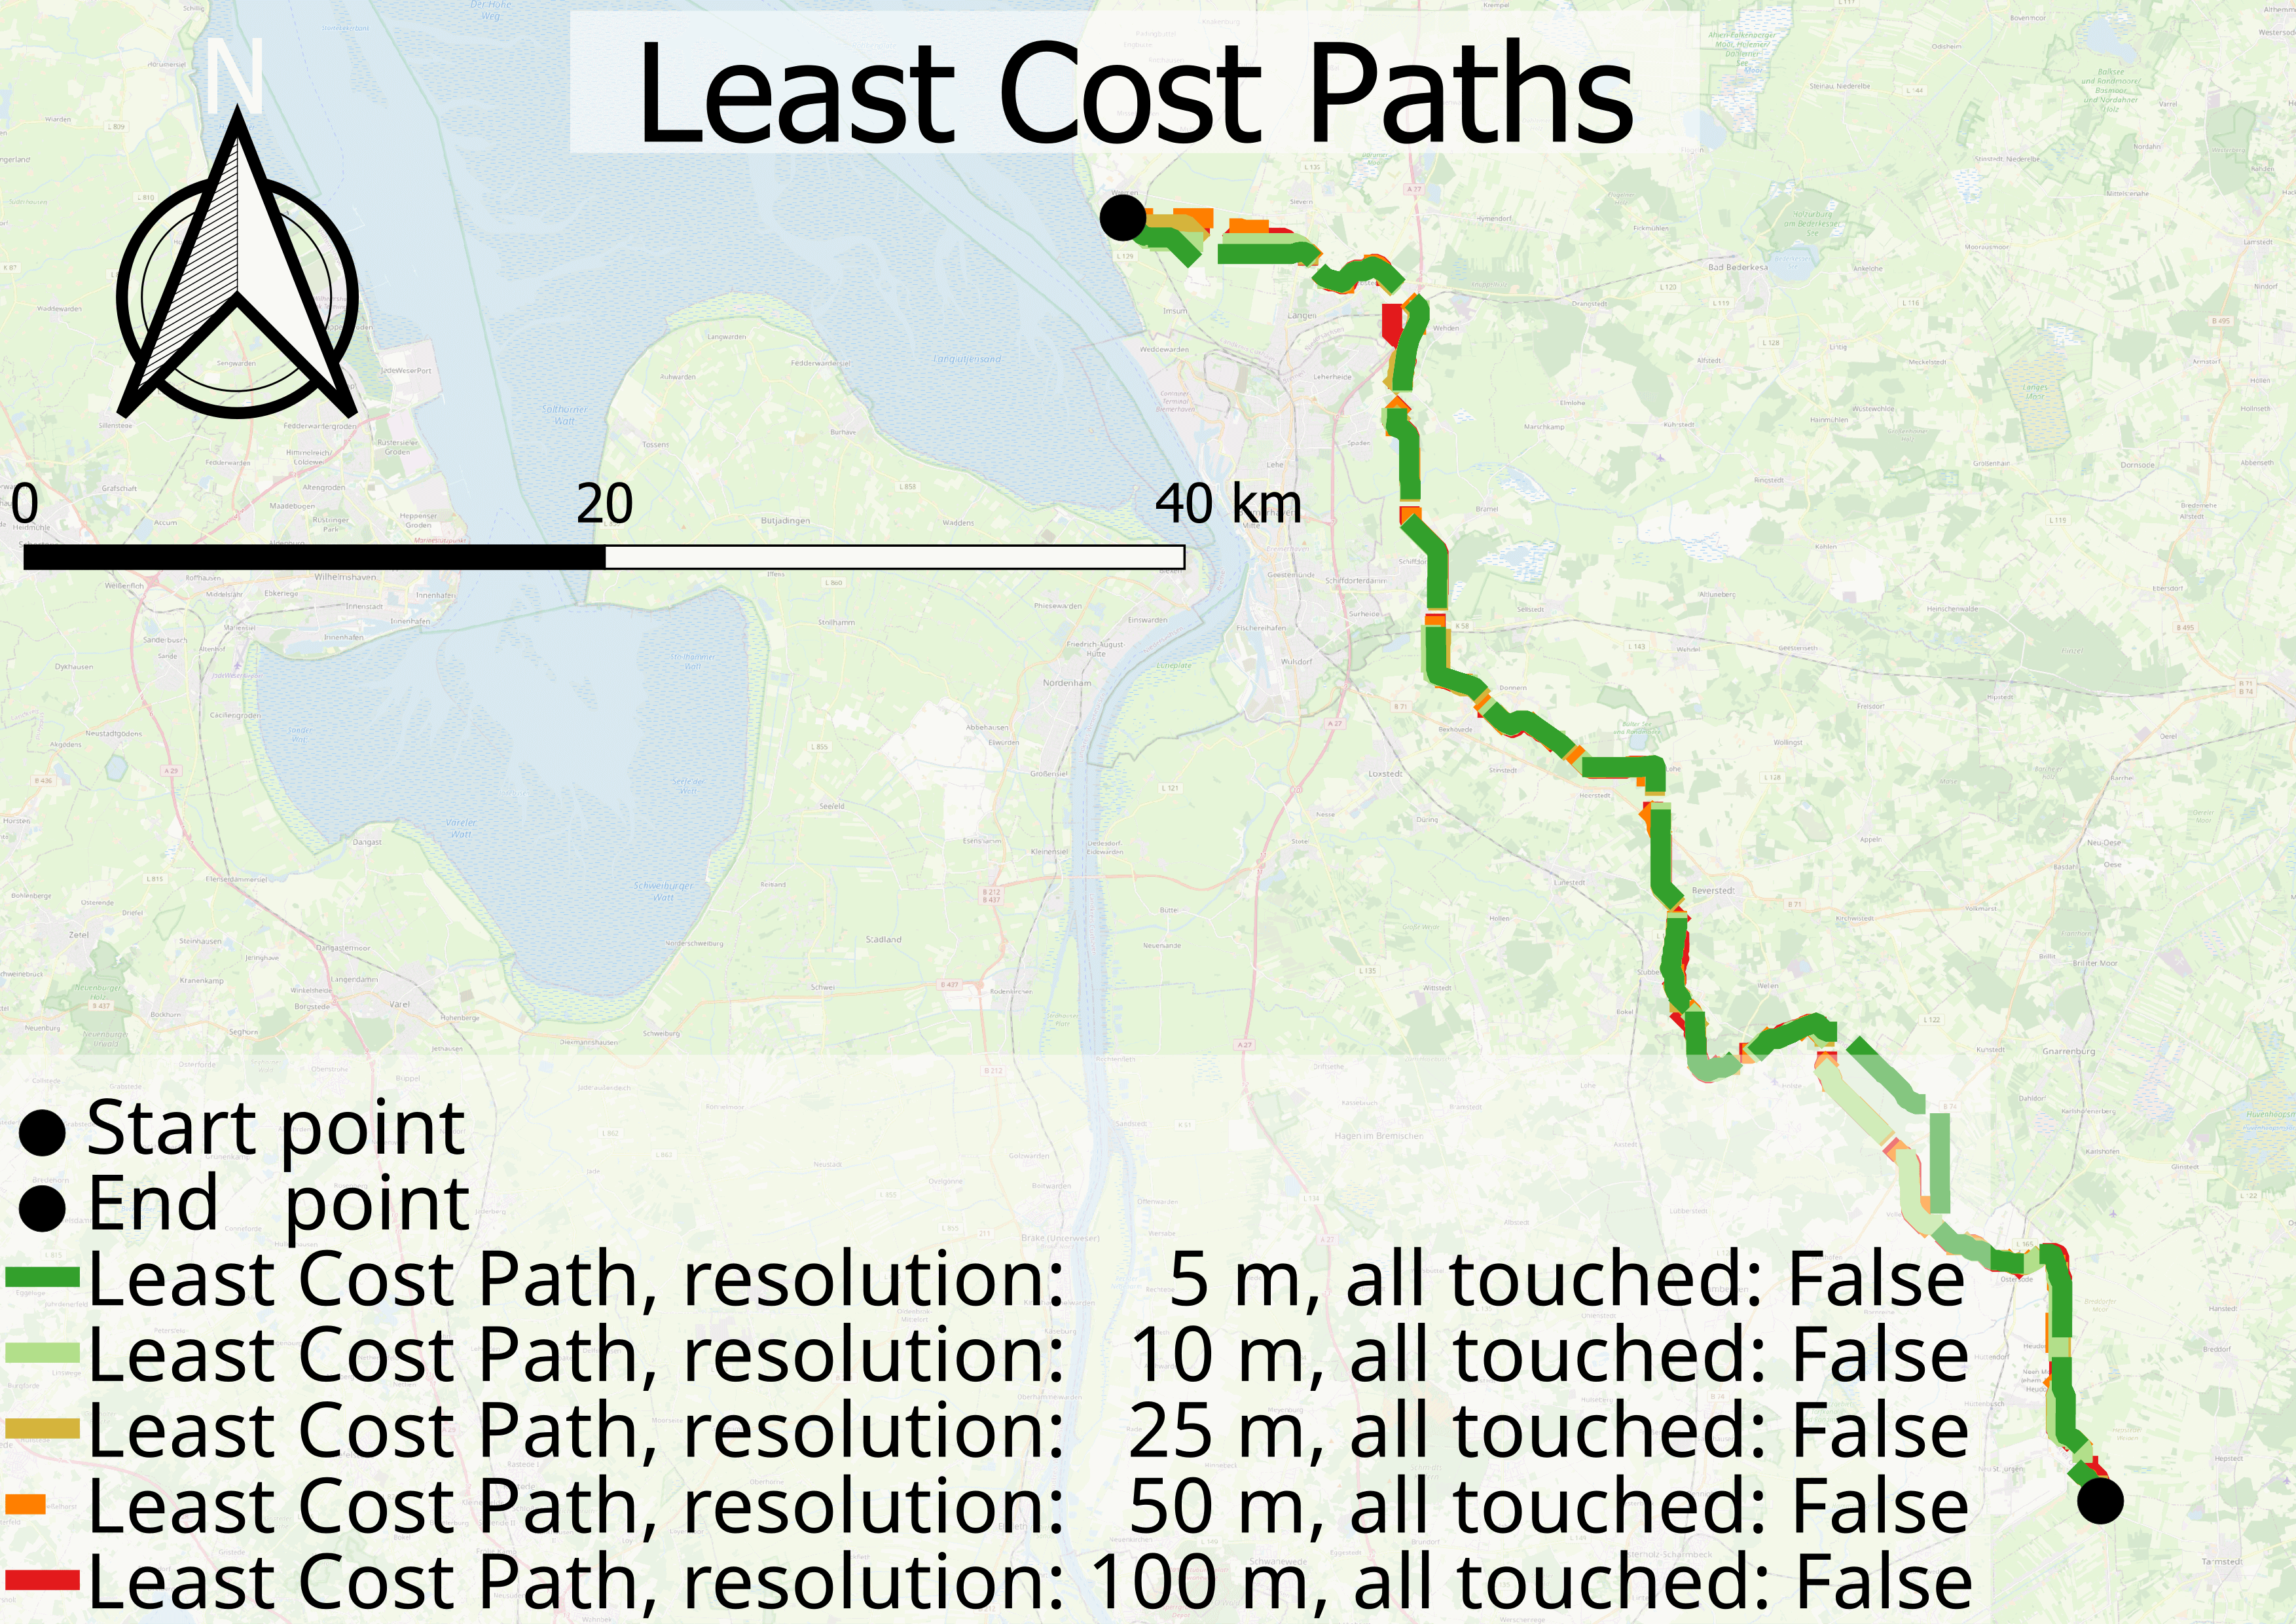
\includegraphics[width=.45\linewidth]{./images/LeastCostPaths_al_F_v2_small.png} }}%
	\qquad
	\subfloat[\centering all touched True.]{{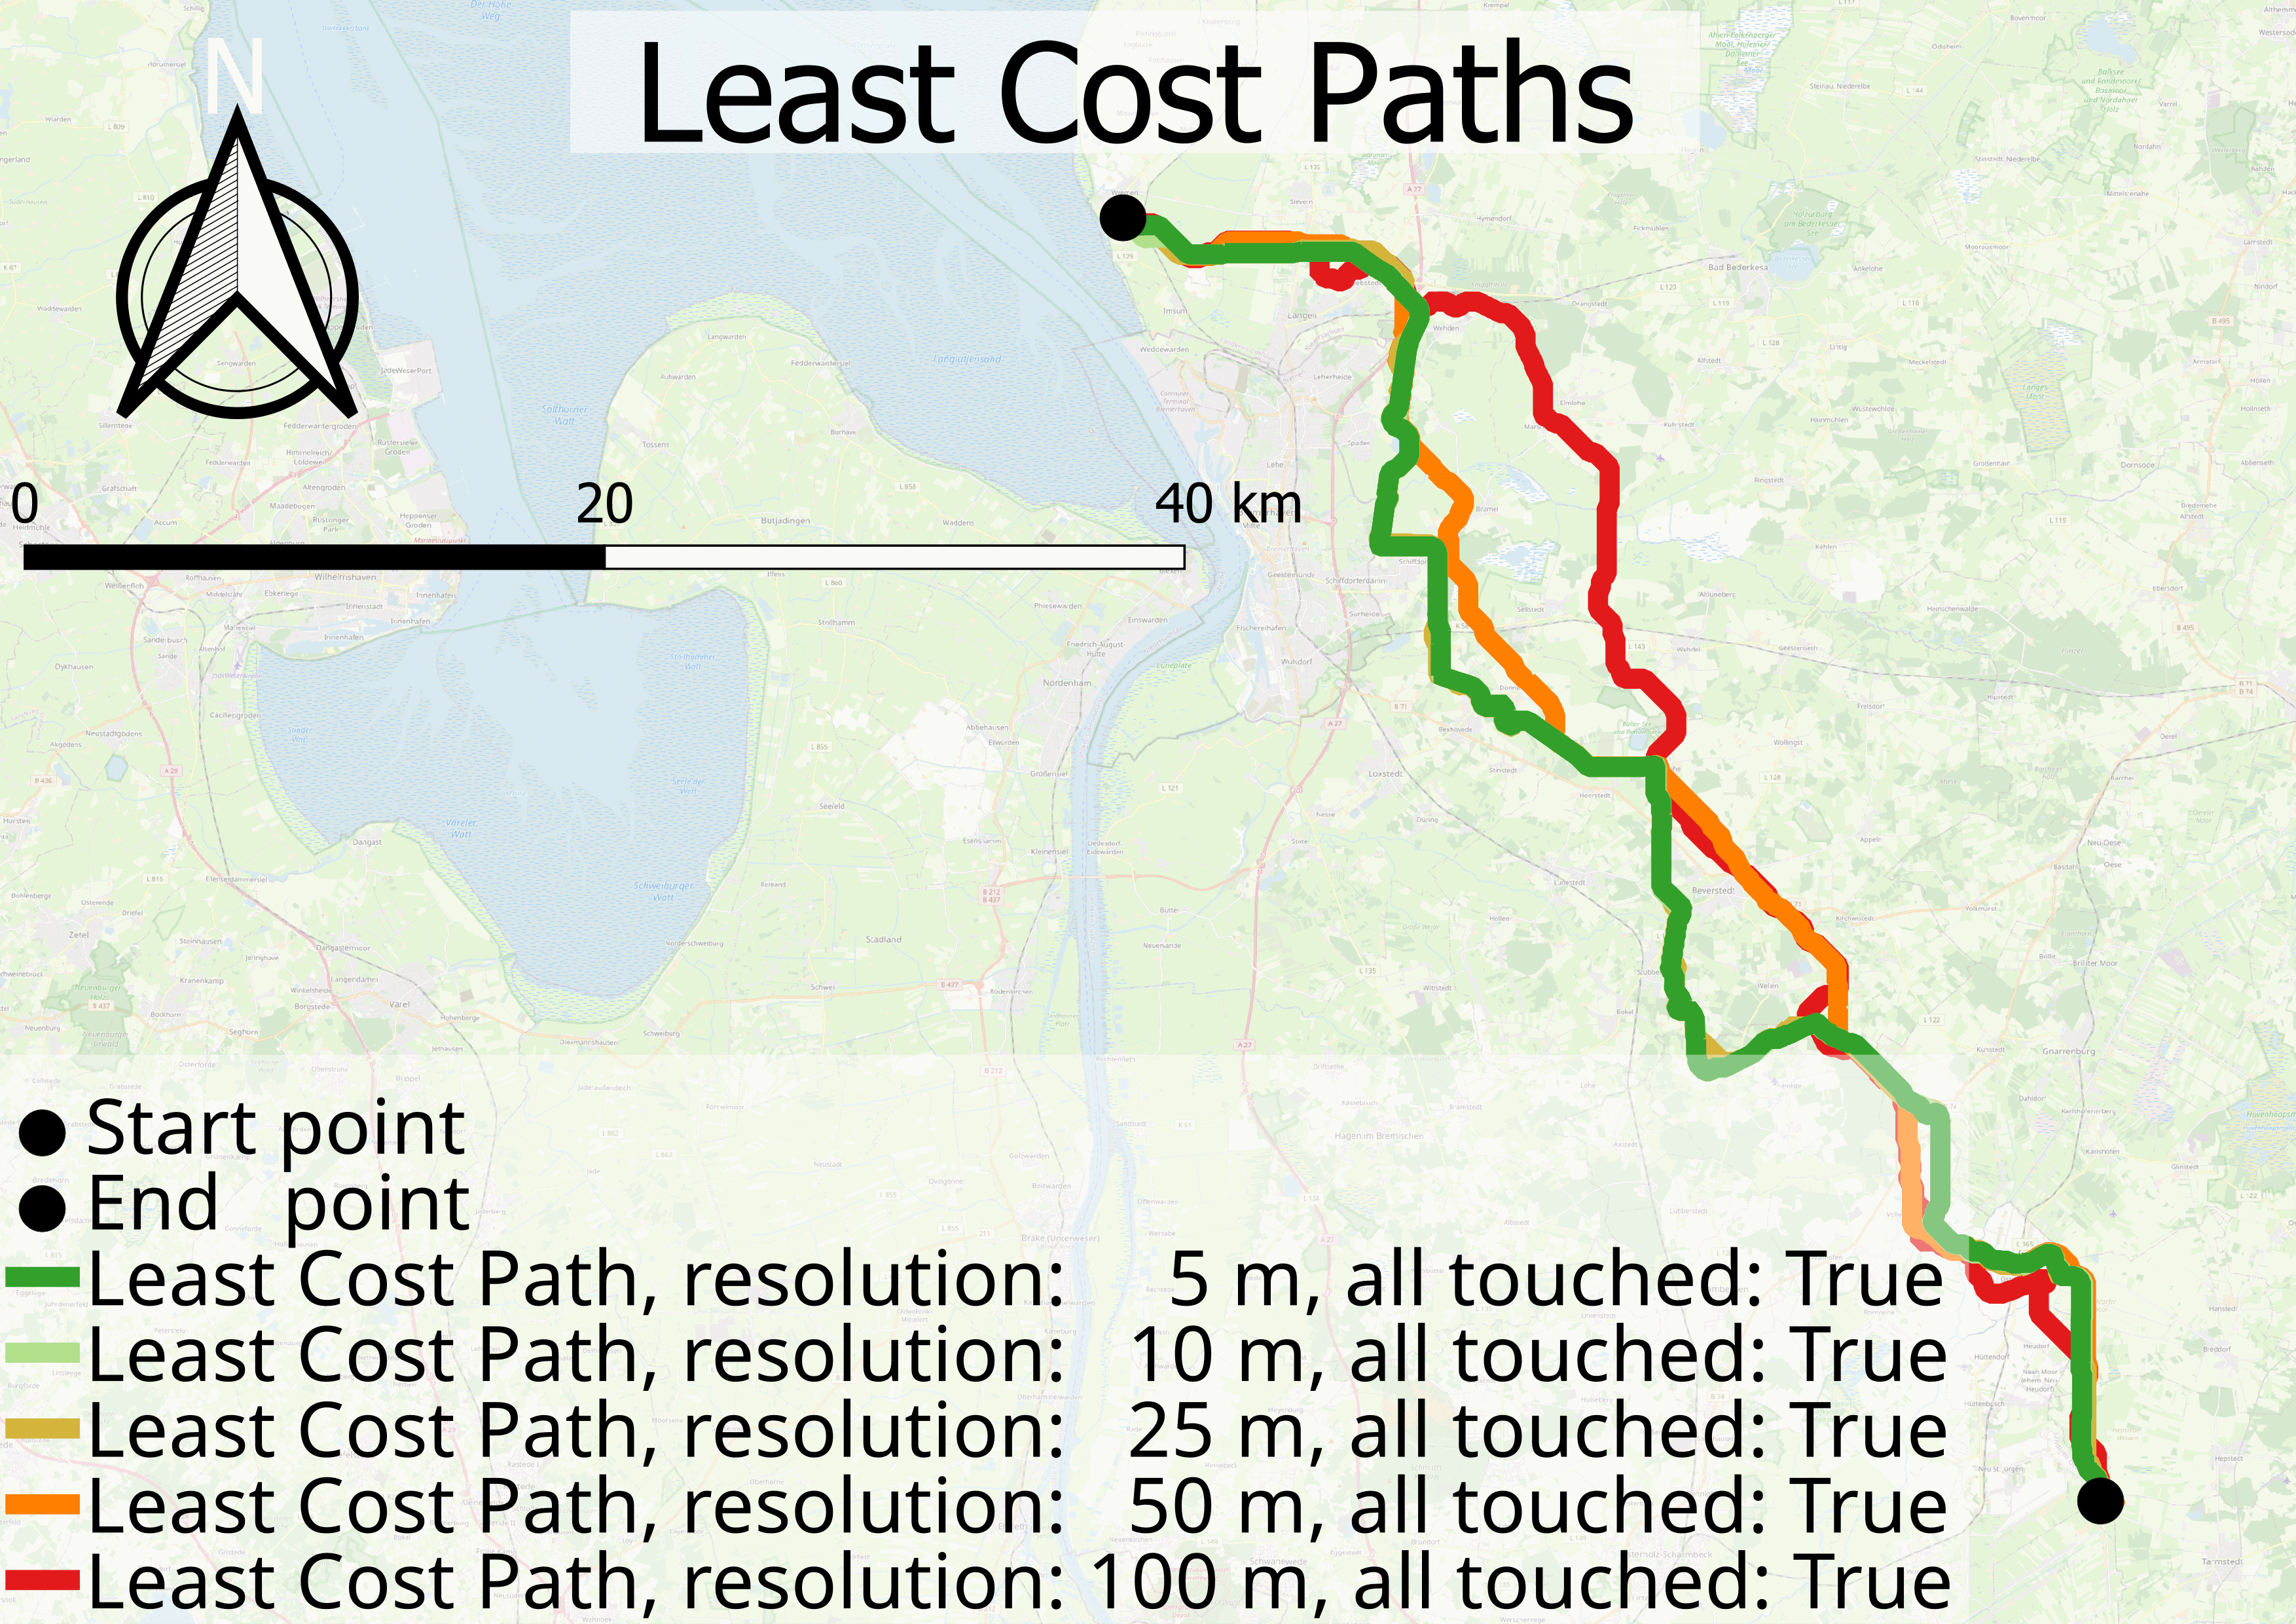
\includegraphics[width=.45\linewidth]{./images/LeastCostPaths_al_T_v2_small.png} }}%

	\caption{Figures of the Least Cost Paths contrasting the changes of the Least Cost Paths for the different results, depending on the parameter all~touched. Paths setting all~touched to False are indicated by dashed lines and True are indicated by continuous lines. Higher resolutions are indicated by the color green, lower resolutions by the color red. Using OpenStreetMaps as base map.}
	\label{fig:paths_alltouched}
\end{figure}

\begin{table*}[t]
	\caption{Least Cost Paths as length~(l) for the different resolutions~(res), including the mean minimum distance~($d_{mean}$) and the maximum minimum distance~($d_{max}$) and the agg. costs. From the agg. costs the differences of the agg. costs and the agg. costs per resolution are computed.} 
	\label{tab:2}
	\centering
	\begin{tabular}{ r  r  r  r  r  r  r  r  r  r}
		res /m & $l_{al=f} /m$ & $l_{al=t} /m$ & $d_{mean}$ /m & $d_{max}/m$ & agg.  $ cost_{al=f}$ & agg. $ cost_{al=t}$ &  $\Delta $ costs & agg. $costs_{al=f} /m$ & agg. $costs_{al=t} /m$ \\
		\hline
		5 	& 76136.3	& 78002.0 &  126.0 & 1065.0 & 18665.9 & 19616.8 & -850.00 & 93329.6 &  97584.8 \\
		10 	& 75430.1 	& 77936.6 &  277.9 & 1590.0 &  8931.2 &  9731.2 & -799.95 & 89312.5 &  97311.8 \\
		25 	& 75422.9 	& 78422.9 &  313.8 & 1621.2 &  3354.9 &  3872.7 & -517.78 & 83871.7 &  96816.4 \\
		50 	& 76135.0	& 70620.0 & 1140.0 & 4950.0 &  1409.0 &  2300.1 & -891.05 & 70451.2 & 115003.7 \\
		100 & 76283.8	& 74120.7 & 1946.4 & 6016.6 &   640.5 &  1572.3 & -931.70 & 64051.6 & 167226.8 \\

	\end{tabular}
\end{table*}

When estimating the distance between the Least Costs Paths from all~touched set to True and all~touched set to False at the same resolution, 
the mean minimum distance between the 100~m resolution paths is 1946.41~m and between the 5~m resolution paths is 126.04~m.
The similarity between the all~touched set to False paths is higher, than for setting to True.
The distance for the 100~m path to the 5~m resolution path is 243.42~m for all~touched False and 2109.44~m for all~touched True.

When cross comparing the similarity between all paths set with all~touched set to False and the similarity in between the same resolution, the similarity in between the all~touched set to False paths is higher, than for most paths of the same resolution.
Namely except for the highest resolution.

This behaviour is shown in figure~\ref{fig:paths_alltouched}.
On a more detailed level, it can be seen, that the paths of all~touched False also converge directly to the all~touched True paths, but the extent is smaller.


The zonal stat (see table~\ref{tab:3}) for a buffer of 100~m (5~m) around the paths has been used, to estimate the
percentage of each costs levels around the paths.
When using all~touched True at higher resolution the tendency is to use a higher percentage of the
\textit{Preferential} Level and less of the \textit{NoRestriction} Level.
There is no strong tendency for the all~touched set to False Least Cost Paths.

\setlength{\tabcolsep}{10pt}

\begin{table*}[t]
	\caption{Resolution (res) of category percentages of each Least Cost Path for a buffer of 100 m (5 m) around the Least Cost Path for each raster reprojected to 5~m resolution.}
	\label{tab:3}
	\centering
	\begin{tabular}{ r  r  r r  r r  r r  r r  r r}
		res /m & all touched & \multicolumn{2}{c}{ $ r_{Preferential} \% $}  & \multicolumn{2}{c}{ $ r_{No Restriction} \% $ }  & \multicolumn{2}{c}{ $ r_{Restricted} \% $}  & \multicolumn{2}{ c }{ $ r_{strongly Restricted}\% $ } & \multicolumn{2}{c}{ $ r_{Prohibited} \% $ } \\
		\hline
		5 & False &  4.7  &  (5.4) & 58.7 & (58.9) & 8.8 & (8.4) & 0.7 & (0.7) & 27.1 & (26.7)  \\
		10 & False &  19.6 & (33.5) & 68.5 & (64.5)  & 1.0 & (0.8) & 0.8 & (0.3) & 10.1 & (0.9)\\
		25 & False &  19.2 & (34.2) & 68.9 & (64.9)  & 1.0 & (0.2) & 0.7 & (0.1) & 9.7 & (0.6)\\
		50 & False &  20.4 & (33.2) & 68.0 & (66.2)  & 0.9 & (0.1) & 0.7 & (0.0) & 10.1 & (0.5)\\
		100 & False &  21.1 & (30.7) & 69.1 & (68.8)  & 1.1 & (0.0) & 0.7 & (0.0) & 7.9 & (0.4) \\

		\hline

		5 & True  &  18.9 & (28.5) & 67.3 & (66.4) & 1.3 & (1.6) & 1.0 & (0.5) & 11.5 & (3.0) \\	
		10 & True &  18.9 & (33.7) & 66.6 & (63.4)  & 1.6 & (1.4) & 1.4 & (0.6) & 11.5 & (1.0)\\	
		25 & True &  18.7 & (31.9) & 65.5 & (65.5)  & 2.0 & (1.3) & 2.5 & (0.7) & 11.4 & (0.6)\\
		50 & True &  9.1 & (13.0) & 75.7 & (83.0) & 3.9 & (2.0) & 4.2 & (1.6) & 7.1 & (0.4) \\
		100 & True &  7.0 & (10.1) & 73.8 & (81.9)  & 5.5 & (3.9) & 8.5 & (3.6) & 5.2 & (0.4) \\	
	\end{tabular}
\end{table*}


\subsection{Execution time}\label{subsec:execution-time}

In theory, the execution time increases by power of two with the resolution, because higher resolutions result in a higher number of pixels. 
A double logarithmic fit shows, that the execution time scales with power of $2.1997  \pm 0.007$ of the inverse resolution. 

The total execution time consists of two parts:
the aggregation of the costs and the back tracking of the least cost to find the path.


\subsection{Faster Processing of the Cost Path Algorithm}\label{subsec:faster-processing-of-the-cost-path-algorithm}

The first step is to optimise the computational speed by a reduced area.
Another method is to improve the prediction of the medium resolution itself and thus reduce the need for a computation in higher resolution.

\subsubsection{Compare Least Cost Paths from rasters of both all~touched settings}

For the example paths shown, all~touched set to True overestimates ans set to False underestimates the True costs.

A weighted average of the costs could therefore be a more accurate measure and make estimated medium resolution Least Cost Path more similar to high resolution paths.
As above example shows the weighting should favour all~touched to False.

This will speed-up the aggregation.
The time needed for the back tracking stays unchanged.

The optimal ratio of overlaying both all~touched for cost raster with 10~m resolution is estimated via similarity of the resulting Least Cost Path to the path of the original high resolution raster. 
The mean distance of Least Cost Paths from rasters with different ratio is estimated to the path from the all~touched set to False raster of the higher (5~m) resolution. 
Table~\ref{tab:4} shows, that the mean minimum distance decreases with increasing ratio (1:1, 2:1, 4:1) and after this optimum is reached, increases with increasing ratio (8:1, 16:1 and so on).
Comparing  the similarity of the paths of the different ratios to normal paths with 10~m resolution shows, that paths with a higher ratio of all~touched set to True are nearer to the all~touched set to True paths.
Paths with a ratio in favour of all~touched False are much closer to the all~touched set to False paths.


\begin{table}[h!]
	\caption{Paths computed from the overlaying of all~touched set to False and True raster with the mean minium distance (d) of the paths to the paths calculated from the all~touched set to False 5~m resolution and all~touched set to False and True raster at 10~m resolution with the ratio (r).}
	\label{tab:4}
	\centering
	\begin{tabular}{ r  r  r  r}
		r & $d_{5~al=f}$ /m &  $d_{10~al=f}$ /m & $d_{10~al=t}$ /m \\
		\hline
		
		  1:1  &    119.6 &  285.5 &  47.2\\
		  2:1  &    97.1 &  263.5 &  74.2\\
		  4:1  &    40.1 &  206.4 & 100.2\\
		  8:1  &    41.7 &  169.0 & 137.3\\
		 16:1  &    56.7 &  153.3 & 152.72\\
		 32:1  &    56.7 &  145.6 & 162.1\\
		 64:1  &   163.5 &   10.6 & 272.4\\
	  % 128:1  &   163.80 &   10.3 & 276.7\\
		
	\end{tabular}
\end{table}


\subsubsection{Compare Least Cost Paths from downsampled cost raster}

As an alternative to the superposition of the rasters of same resolution, a high resolution (5~m) all~touched False raster is downsampled to 10~m, 25~m, 50~m and 100~m (bi-linear) interpolation.

The distances from the paths that are computed from the bi-linear downsampled raster to the path of the original 5~m resolution (all~touched False) shows, that only downsampling to a resolution of 10~m produces a path that is relatively close the high resolution paths(see table~\ref{tab:5}).

The opposite is True for the lower resolution raster which is more similar to paths computed from the all~touched True cost raster.
Every path from a downsampled raster is more similar to a path computed from an all~touched set to True raster, than to an all~touched set to False raster, although the all~touched set to False raster of the 5 m resolution was used for downsampling.\todo{interpretation all~touched True and downsampling, both show all details, but downsampling, more similar to original geometry}

\begin{table}[h!]
	\caption{Length (l) of the path computed from the bi-linear downsampled raster and the mean minimum distance (d) of the paths from the downsampled raster to the paths calculated from the all~touched set to True and False raster of the same resolution as the downsampled raster with resolution (res).}
	\label{tab:5}
	\centering
	\begin{tabular}{ r  r  r  r  r}
		res /m & l /m  & $d_{5~m}$ /m &  $d_{al=f}$ /m & $d_{al=t}$ /m \\
		\hline
		
		10  & 75980.6 &    59.3 &  219.4 & 143.6\\
		25  & 70205.3 &   385.8 &  558.1 & 432.8\\
		50  & 69217.9 &   730.8 &  693.4 & 255.7\\
		100 & 66667.9 &  1681.3 & 1605.6 & 400.6\\
		
	\end{tabular}
\end{table}


% \subsubsection{Restrict search to a minimum sized bounding box}
\subsubsection{Restrict search to a buffer around the Least Cost Paths}



Construct a polygon from the two Least Cost Paths (all~touched True and all~touched False of the same resolution).
Buffer the polygon with twice the maximum  minimum path distance  (see equation~\ref{eq:2}).
\begin{equation}
	\label{eq:2}
	d_{max} = max(\sum_{i=1}^{n} d_{min}(P_i, L_2)) \Bigr\vert P_i \in L_1
\end{equation}

This strategy results in the same Least Cost Path as with the original high resolution raster.

This reduction of compute power provides the possibility  to run a 2.5~m.
This clipped 2.5~m raster for all~touched set to True changes the path only slightly. 

The all~touched False raster, on the other hand, leads to a completely new previously unused subroute at the end of the path.
Due to the low resolution a small path became passable.
This small path is a power line next to a road between protected landscape areas.
The road and the protected landscape areas are both \textit{restricted} areas, while the power line is \textit{preferred}.



%\subsubsection{Restrict search to reachable points}
%For this purpose the aggregated cost as to converted back into a raster.

\subsubsection{Apply the proposed solutions on other paths}
To broaden the view and verify the result, four different routes should be found using the above strategies.
Two routes should be found from the starting point to two new points in the south east of the investigated area and two routes should be found from the north and north east of the study area to the end point.

For three of the four routes, the Least Cost Path estimation from the clipped raster was able to calculate exactly the same result.
For the fourth path, the Least Cost Path from the 5~m resolution raster was clipped by the buffer around the 50~m resolution paths.
The speed up from the clipping of the higher resolution raster depends on the number of pixels that have been clipped. 

Bi-linear downsampling the of the high resolution raster to a medium resolution did not result in any benefits compared to an original medium resolution raster.
The aggregated cost per resolution of the Least Cost Path from the downsampled raster is higher than the normal medium resolution 10~m raster.
In addition, the distance from these paths to the high resolution path  is greater than the distance from the original 10~m resolution path to the 5~m resolution path (see table~\ref{tab:6}).
\todo{interpretation: Why is the downsampling result so different? Don't know.}

\begin{table}[h!]
	\caption{Length (l) of the path, the aggregated costs per resolution and the mean minimum distance ($d_{mean}$) to the path created from the 5~m resolution all~touched False raster for the four control routes, for the reference path constructed from the 5~m  and 10~m raster and the from 5~m to 10~m downsampled raster and the 5~m clipped raster for the routes point1 to end point (P1-E), point2 to end point (P2-E), start point to point3 (S-P3) and start point to point4 (S-P4).}
	\label{tab:6}
	\centering
	\begin{tabular}{ r @{\hspace*{3mm}}  r  r  r  r}
		Route & Method & $length /m$ & $costs_{al=f}$ & $d_{mean}$ /m \\
		\hline
		P1-E & 5~m 			& 107889.6 & 208547.8 &        \\
		 	 & Clipped 		& 107889.6 & 208547.8 &   0.0  \\
		 	 & Down			&  96754.2 & 212911.0 & 628.1 \\
		 	 & 10~m 		& 107232.9 & 203010.2 & 103.5 \\
		\hline
		P2-E & 5~m 			& 103706.4 & 155567.9 &        \\
		 	 & Clipped 		& 103706.4 & 155567.9 &   0.0 \\
		 	 & Down 	    &  92403.3 & 158238.6	& 639.9 \\
		 	 & 10~m 		& 104249.9 & 149899.7 & 177.7 \\
		\hline
		S-P3 & 5~m 			& 102187.1 & 34503.8 	&         \\
			 & Clipped 		&  90377.1 & 37926.1 	& 4465.4 \\
			 & Down 	    &  94125.6 & 37574.9 	&  742.4 \\
			 & 10~m 		& 102461.6 & 32446.0 	&   81.2 \\
		\hline
		S-P4 & 5~m 			& 96449.2 	& 33865.5 	&  		\\
		 	 & Clipped 		& 96449.2 	& 33865.5 	& 0.0 	\\
			 & Down 		& 87861.1 	& 36462.7 	& 796.4\\
			 & 10~m 		& 96739.5 	& 31899.3	& 83.5 \\

		
	\end{tabular}
\end{table}



